\chapter{Графты аралау}

Бұл тарау екі негізгі граф алгоритмдері туралы болмақ.
Біріншісі -- тереңдігі бойынша іздеу, екіншісі -- ені бойынша іздеу. 
Екі алгоритмде де алғашында графтағы бастапқы төбе беріледі және олар бастапқы төбеден жете алатын барлық төбелерге барып шығады.
Алгоритмдердің айырмашылығы төбелерге келу реттілігіне байланысты туындайды.
% The difference in the algorithms is the % order
% in which they visit the nodes.

\section{Тереңдігі бойынша іздеу}

\index{тереңдігі бойынша іздеу}

\key{Тереңдігі бойынша іздеу} (DFS) --
қарапайым графты өтіп шығу әдісі.
Алгоритм алғашқы төбеден бастап, графтағы қырларды қолдана отырып, басқа төбелерге жетеді.

Тереңдігі бойынша іздеу әрқашан бастапқы төбеден басталады және басқа бармаған төбелерге апаратын қыр болса, сол төбелерге тікелей жалғасады. Ал егер бармаған басқа төбеге апаратын жол болмаса, кейін қайтып, артынша бармаған басқа төбелерге қарай өтеді.
Алгоритм әрбір төбеге тек бір рет қана бару үшін жеткен төбелерін сақтап отырады.

\subsubsection*{Мысал}

Төменде берілген графты тереңдігі бойынша өтіп көрейік:
\begin{center}
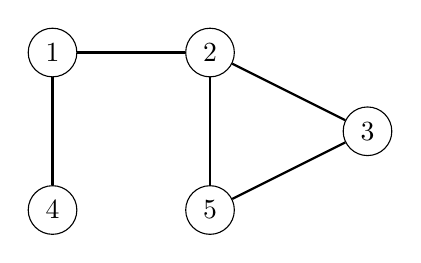
\begin{tikzpicture}
\node[draw, circle] (1) at (1,5) {$1$};
\node[draw, circle] (2) at (3,5) {$2$};
\node[draw, circle] (3) at (5,4) {$3$};
\node[draw, circle] (4) at (1,3) {$4$};
\node[draw, circle] (5) at (3,3) {$5$};

\path[draw,thick,-] (1) -- (2);
\path[draw,thick,-] (2) -- (3);
\path[draw,thick,-] (1) -- (4);
\path[draw,thick,-] (3) -- (5);
\path[draw,thick,-] (2) -- (5);
\end{tikzpicture}
\end{center}
Біз ізденісті кез келген төбеден бастай аламыз. Келтіріліп отырған мысалда біз $1$-төбеден бастаймыз.

Бірінші, ізденіс $1$-төбеден $2$-төбеге жетеді:
\begin{center}
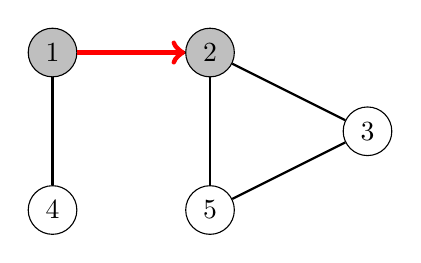
\begin{tikzpicture}
\node[draw, circle,fill=lightgray] (1) at (1,5) {$1$};
\node[draw, circle,fill=lightgray] (2) at (3,5) {$2$};
\node[draw, circle] (3) at (5,4) {$3$};
\node[draw, circle] (4) at (1,3) {$4$};
\node[draw, circle] (5) at (3,3) {$5$};

\path[draw,thick,-] (1) -- (2);
\path[draw,thick,-] (2) -- (3);
\path[draw,thick,-] (1) -- (4);
\path[draw,thick,-] (3) -- (5);
\path[draw,thick,-] (2) -- (5);

\path[draw=red,thick,->,line width=2pt] (1) -- (2);
\end{tikzpicture}
\end{center}
Содан кейін $3$ және $5$-төбелерге барады:
\begin{center}
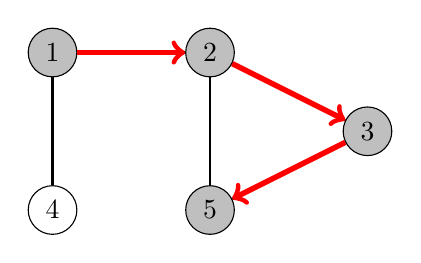
\begin{tikzpicture}
\node[draw, circle,fill=lightgray] (1) at (1,5) {$1$};
\node[draw, circle,fill=lightgray] (2) at (3,5) {$2$};
\node[draw, circle,fill=lightgray] (3) at (5,4) {$3$};
\node[draw, circle] (4) at (1,3) {$4$};
\node[draw, circle,fill=lightgray] (5) at (3,3) {$5$};

\path[draw,thick,-] (1) -- (2);
\path[draw,thick,-] (2) -- (3);
\path[draw,thick,-] (1) -- (4);
\path[draw,thick,-] (3) -- (5);
\path[draw,thick,-] (2) -- (5);

\path[draw=red,thick,->,line width=2pt] (1) -- (2);
\path[draw=red,thick,->,line width=2pt] (2) -- (3);
\path[draw=red,thick,->,line width=2pt] (3) -- (5);
\end{tikzpicture}
\end{center}
$5$-төбенің көршілері -- $2$ және $3$-төбелер. Бірақ біз бұл төбелерде әлдеқшан болғандықтан оларға бара алмай, артқы төбеге қайтамыз.
Сондай-ақ $3$, $2$-төбелердің көршілеріне де бұған дейін барып қойғандықтан, біз $1$-төбеге қайтамыз. Осылайша $4$-төбеге де жетеміз:
\begin{center}
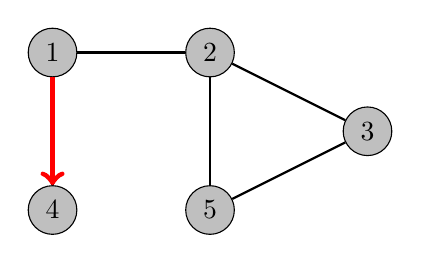
\begin{tikzpicture}
\node[draw, circle,fill=lightgray] (1) at (1,5) {$1$};
\node[draw, circle,fill=lightgray] (2) at (3,5) {$2$};
\node[draw, circle,fill=lightgray] (3) at (5,4) {$3$};
\node[draw, circle,fill=lightgray] (4) at (1,3) {$4$};
\node[draw, circle,fill=lightgray] (5) at (3,3) {$5$};

\path[draw,thick,-] (1) -- (2);
\path[draw,thick,-] (2) -- (3);
\path[draw,thick,-] (1) -- (4);
\path[draw,thick,-] (3) -- (5);
\path[draw,thick,-] (2) -- (5);

\path[draw=red,thick,->,line width=2pt] (1) -- (4);
\end{tikzpicture}
\end{center}
Бұдан кейін ізденіс бітеді. Себебі біз барлық төбелерде болдық.

Төбелердің санын $n$, ал қырлардың санын $m$ деп белгілесек, бұл алгоритмнің уақытша күрделілігі $O(n+m)$-ге тең болады. Себебі алгоритм әр төбені және әр қырды бір рет өтіп шығады.

\subsubsection*{Кодтың жазылуы}

Тереңдiгi бойынша iздеу алгоритмін рекурсия арқылы жазу ең оңай әдіске жатады. Төмендегі \texttt{dfs} функциясында бастапқы төбені қабылдаймыз. Сол төбеден ізденісті бастаймыз. Бұл ізденіс функциясында біз cыбайластық тізімімен жұмыс жасаймыз:
\begin{lstlisting}
vector<int> adj[N];
\end{lstlisting}
Сондай-ақ барған төбелерді жиымда сақтаймыз:
\begin{lstlisting}
bool visited[N];
\end{lstlisting}
Алғашында жиымдағы әр элемент \texttt{false} болады. Ал $s$ төбесіне келгенде \texttt{visited}[$s$] элементі \texttt{true} болып өзгереді.
Бұл функцияны төмендегідей етіп жазуға болады:
\begin{lstlisting}
void dfs(int s) {
    if (visited[s]) return;
    visited[s] = true;
    // process node s
    for (auto u: adj[s]) {
        dfs(u);
    }
}
\end{lstlisting}

\section{Ені бойынша іздеу}

\index{ені бойынша іздеу}

\key{Ені бойынша іздеуде} (BFS) графтың төбелеріне бастапқы төбеден арақашықтың өсу ретіне қарай барылады. Алгоритм арқылы бастапқы төбе мен графтағы кез келген төбе арасындағы арақашықтықты есептеу оңайға соғады. Бірақ кодтың жазылуы тереңдігі бойынша ізденістен қиынырақ болады.

Ізденіс барысында төбелерді кезең-кезеңімен өтіп шығамыз.
Алдымен бастапқы орнымыздан 1 қыр арақашықтығындағы барлық төбелерден өтеміз,
кейін арақашықтығы 2 болатын төбелерге барамыз. Бұл үдеріс барлық төбелерді өтіп шыққанға дейін жалғаса береді.

\subsubsection*{Мысал}

Мысалға төмендегі графты қарастырайық:

\begin{center}
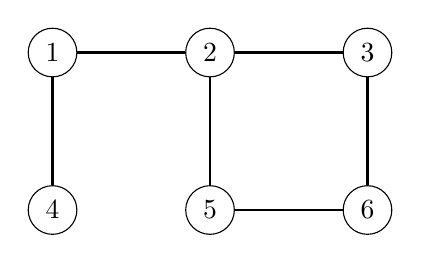
\begin{tikzpicture}
\node[draw, circle] (1) at (1,5) {$1$};
\node[draw, circle] (2) at (3,5) {$2$};
\node[draw, circle] (3) at (5,5) {$3$};
\node[draw, circle] (4) at (1,3) {$4$};
\node[draw, circle] (5) at (3,3) {$5$};
\node[draw, circle] (6) at (5,3) {$6$};

\path[draw,thick,-] (1) -- (2);
\path[draw,thick,-] (2) -- (3);
\path[draw,thick,-] (1) -- (4);
\path[draw,thick,-] (3) -- (6);
\path[draw,thick,-] (2) -- (5);
\path[draw,thick,-] (5) -- (6);
\end{tikzpicture}
\end{center}
Ені бойынша ізденісті $1$-төбеден бастаймыз.
Алдымен біз $1$-төбемен бір қыр арқылы жалғасып тұрған төбелерге барамыз:
\begin{center}
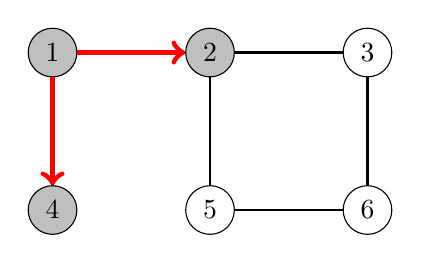
\begin{tikzpicture}
\node[draw, circle,fill=lightgray] (1) at (1,5) {$1$};
\node[draw, circle,fill=lightgray] (2) at (3,5) {$2$};
\node[draw, circle] (3) at (5,5) {$3$};
\node[draw, circle,fill=lightgray] (4) at (1,3) {$4$};
\node[draw, circle] (5) at (3,3) {$5$};
\node[draw, circle] (6) at (5,3) {$6$};

\path[draw,thick,-] (1) -- (2);
\path[draw,thick,-] (2) -- (3);
\path[draw,thick,-] (1) -- (4);
\path[draw,thick,-] (3) -- (6);
\path[draw,thick,-] (2) -- (5);
\path[draw,thick,-] (5) -- (6);

\path[draw,thick,-] (1) -- (2);
\path[draw,thick,-] (2) -- (3);
\path[draw,thick,-] (1) -- (4);
\path[draw,thick,-] (2) -- (5);

\path[draw=red,thick,->,line width=2pt] (1) -- (2);
\path[draw=red,thick,->,line width=2pt] (1) -- (4);
\end{tikzpicture}
\end{center}
Кейін $3$ және $5$-төбелерге жетеміз:
\begin{center}
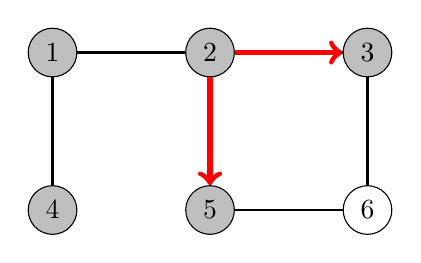
\begin{tikzpicture}
\node[draw, circle,fill=lightgray] (1) at (1,5) {$1$};
\node[draw, circle,fill=lightgray] (2) at (3,5) {$2$};
\node[draw, circle,fill=lightgray] (3) at (5,5) {$3$};
\node[draw, circle,fill=lightgray] (4) at (1,3) {$4$};
\node[draw, circle,fill=lightgray] (5) at (3,3) {$5$};
\node[draw, circle] (6) at (5,3) {$6$};

\path[draw,thick,-] (1) -- (2);
\path[draw,thick,-] (2) -- (3);
\path[draw,thick,-] (1) -- (4);
\path[draw,thick,-] (3) -- (6);
\path[draw,thick,-] (2) -- (5);
\path[draw,thick,-] (5) -- (6);

\path[draw,thick,-] (1) -- (2);
\path[draw,thick,-] (2) -- (3);
\path[draw,thick,-] (1) -- (4);
\path[draw,thick,-] (2) -- (5);

\path[draw=red,thick,->,line width=2pt] (2) -- (3);
\path[draw=red,thick,->,line width=2pt] (2) -- (5);
\end{tikzpicture}
\end{center}
Ал ең соңында біз $6$-төбеге жетеміз:
\begin{center}
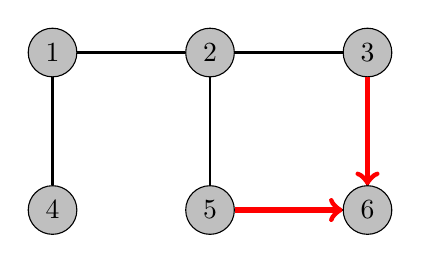
\begin{tikzpicture}
\node[draw, circle,fill=lightgray] (1) at (1,5) {$1$};
\node[draw, circle,fill=lightgray] (2) at (3,5) {$2$};
\node[draw, circle,fill=lightgray] (3) at (5,5) {$3$};
\node[draw, circle,fill=lightgray] (4) at (1,3) {$4$};
\node[draw, circle,fill=lightgray] (5) at (3,3) {$5$};
\node[draw, circle,fill=lightgray] (6) at (5,3) {$6$};

\path[draw,thick,-] (1) -- (2);
\path[draw,thick,-] (2) -- (3);
\path[draw,thick,-] (1) -- (4);
\path[draw,thick,-] (3) -- (6);
\path[draw,thick,-] (2) -- (5);
\path[draw,thick,-] (5) -- (6);

\path[draw,thick,-] (1) -- (2);
\path[draw,thick,-] (2) -- (3);
\path[draw,thick,-] (1) -- (4);
\path[draw,thick,-] (2) -- (5);

\path[draw=red,thick,->,line width=2pt] (3) -- (6);
\path[draw=red,thick,->,line width=2pt] (5) -- (6);
\end{tikzpicture}
\end{center}
Енді біз бастапқы төбеден графтағы барлық төбелерге дейінгі арақашықтықты есептеп шығамыз. Арақашықтықтар төмендегі кестеде көрсетіледі:

\begin{tabular}{ll}
\\
төбе & арақашықтық \\
\hline
1 & 0 \\
2 & 1 \\
3 & 2 \\
4 & 1 \\
5 & 2 \\
6 & 3 \\
\\
\end{tabular}

Тереңдігі бойынша ізденістегідей ені бойынша ізденістің 
уақытша күрделілігі $O(n+m)$. Мұндағы $n$ деп төбелердің санын,
ал $m$ деп қырлардың санын белгілейміз.

\subsubsection*{Кодтың жазылуы}

Ені бойынша ізденіс алгоритмін жазу тереңдік бойынша ізденіс
алгоритмін жазудан қиынырақ. Себебі алгоритм графтың әр жеріндегі төбелер арқылы ретсіз жүреді.
Көбіне бұл алгоритмді төбелердің тізімін сақтайтын кезек деректер құрылымы арқылы жазады.
Әр қадам сайын кезектегі бірінші төбеге барамыз.

Осы ізденіс функциясында cыбайластық тізімін пайдаланамыз, сонымен қатар келесі деректер құрылымдарымен жұмыс жасаймыз:
\begin{lstlisting}
queue<int> q;
bool visited[N];
int distance[N];
\end{lstlisting}

Кодтағы \texttt{q} -- кезек деректер құрылымы, ол төбелердің тізімін
сақтайды. 
\texttt{q} кезегі қашықтықтың өсу ретімен өңделетін төбелерді қамтиды.
Кезектің басында алғашқы төбеге ең жақын,
ал соңына қарай ең алыс төбелер орналасқан. Жаңа бір төбені тізімге қосақан сәтте әрқашан
кезектің соңынан қосамыз, ал келесі баратын төбені тізімнің басынан аламыз. \texttt{visited} жиымы төбеде бұрын болғанымызды немесе болмағанымызды білдіреді. Ал \texttt{distance} жиымы бастапқы төбеден басқа
төбелерге дейінгі арақашықтықты есептейді.

Кодты үлгідегідей етіп жазуға болады ($x$ бастапқы төбе деп алсақ):
\begin{lstlisting}
visited[x] = true;
distance[x] = 0;
q.push(x);
while (!q.empty()) {
    int s = q.front(); q.pop();
    // process node s
    for (auto u : adj[s]) {
        if (visited[u]) continue;
        visited[u] = true;
        distance[u] = distance[s]+1;
        q.push(u);
    }
}
\end{lstlisting}

\section{Қолданыс аясы}

Атап өтілген алгоритмдер арқылы графтың көптеген
қасиеттері туралы ақпарат алуға болады.
Көп жағдайда екі ізденісті де пайдалана аламыз.
Бірақ жазылу жолы оңайырақ болғандықтан, тереңдігі бойынша
ізденіс жиі жасалады. 
Төмендегі қолданыстарда бағытталмаған граф келтірілген деп болжанады.

\subsubsection{Графтың байланыстылығын тексеру}

\index{Байланысты граф}

Егер кез келген екі төбе арасында
жол болса, ол графтың байланыстылығын білдіреді. Демек
біз графтың байланыстылығын кез келген бір
төбені таңдап, одан басқа төбелерге
жете алатындығымызды тексеру арқылы біле аламыз.

Мысалы, төмендегі графта
\begin{center}
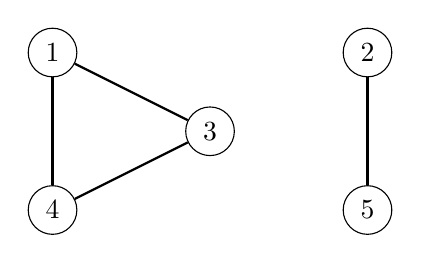
\begin{tikzpicture}
\node[draw, circle] (2) at (7,5) {$2$};
\node[draw, circle] (1) at (3,5) {$1$};
\node[draw, circle] (3) at (5,4) {$3$};
\node[draw, circle] (5) at (7,3) {$5$};
\node[draw, circle] (4) at (3,3) {$4$};

\path[draw,thick,-] (1) -- (3);
\path[draw,thick,-] (1) -- (4);
\path[draw,thick,-] (3) -- (4);
\path[draw,thick,-] (2) -- (5);
\end{tikzpicture}
\end{center}
тереңдігі бойынша ізденісті $1$-төбеден бастасақ,
келесі төбелерге бара аламыз:
\begin{center}
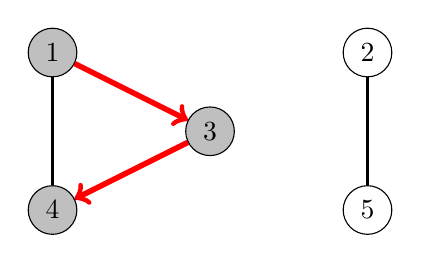
\begin{tikzpicture}
\node[draw, circle] (2) at (7,5) {$2$};
\node[draw, circle,fill=lightgray] (1) at (3,5) {$1$};
\node[draw, circle,fill=lightgray] (3) at (5,4) {$3$};
\node[draw, circle] (5) at (7,3) {$5$};
\node[draw, circle,fill=lightgray] (4) at (3,3) {$4$};

\path[draw,thick,-] (1) -- (3);
\path[draw,thick,-] (1) -- (4);
\path[draw,thick,-] (3) -- (4);
\path[draw,thick,-] (2) -- (5);

\path[draw=red,thick,->,line width=2pt] (1) -- (3);
\path[draw=red,thick,->,line width=2pt] (3) -- (4);

\end{tikzpicture}
\end{center}

Жоғарыдағы мысалдан 1-ші төбеден басталған тереңдігі бойынша іздеу барлық төбелерге бара алмайтынын көреміз. Сондықтан графты өзара
байланыссыз деп қорытынды жасауға болады. Дәл осылай графтың  барлық компоненттерін таба аламыз. Ол үшін барлық төбелерді өтіп шығып, егер ағымдағы төбе бұған дейін табылған байланыстылық компонентінің бір де біреуіне жатпаса, тереңдігі бойынша жаңа іздеуді бастаймыз.  

\subsubsection{Циклдарды табу}

\index{цикл}

Егер біз графтың тереңдігі бойынша ізденіс жасап келе жатып, сол сәтте тұрақтаған
ағымдағы төбенің көршісі осыған дейін өтілгенін байқасақ, граф циклды қамтыды деп санаймыз.
Мысалға, келесі граф екі циклды қамтиды:
\begin{center}
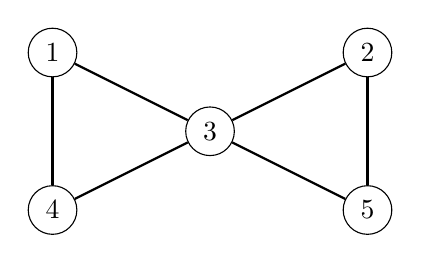
\begin{tikzpicture}
\node[draw, circle] (2) at (7,5) {$2$};
\node[draw, circle] (1) at (3,5) {$1$};
\node[draw, circle] (3) at (5,4) {$3$};
\node[draw, circle] (5) at (7,3) {$5$};
\node[draw, circle] (4) at (3,3) {$4$};

\path[draw,thick,-] (1) -- (3);
\path[draw,thick,-] (1) -- (4);
\path[draw,thick,-] (3) -- (4);
\path[draw,thick,-] (2) -- (5);
\path[draw,thick,-] (2) -- (3);
\path[draw,thick,-] (3) -- (5);
\end{tikzpicture}
\end{center}
Төменде циклдардың біреуінің табу жолы көрсетілген:
\begin{center}
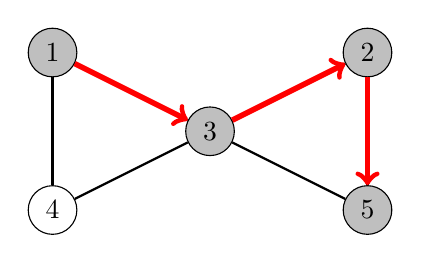
\begin{tikzpicture}
\node[draw, circle,fill=lightgray] (2) at (7,5) {$2$};
\node[draw, circle,fill=lightgray] (1) at (3,5) {$1$};
\node[draw, circle,fill=lightgray] (3) at (5,4) {$3$};
\node[draw, circle,fill=lightgray] (5) at (7,3) {$5$};
\node[draw, circle] (4) at (3,3) {$4$};

\path[draw,thick,-] (1) -- (3);
\path[draw,thick,-] (1) -- (4);
\path[draw,thick,-] (3) -- (4);
\path[draw,thick,-] (2) -- (5);
\path[draw,thick,-] (2) -- (3);
\path[draw,thick,-] (3) -- (5);

\path[draw=red,thick,->,line width=2pt] (1) -- (3);
\path[draw=red,thick,->,line width=2pt] (3) -- (2);
\path[draw=red,thick,->,line width=2pt] (2) -- (5);

\end{tikzpicture}
\end{center}
Мұндағы $2$-төбеден $5$-төбеге жеткен кезде $3$-төбеге әлдеқашан барылғанын
байқаймыз. Сондықтан бұл граф $3$-төбеден өтетін циклды қамтиды.
Мысалға, $3 \rightarrow 2 \rightarrow 5 \rightarrow 3$.

Графта цикл бар екенін басқа жолмен де тексеруге болады. Ол үшін біз
жай ғана әр компоненттегі төбелер мен қырлардың санын есептейміз.
Егер компонентте $c$ төбе болса, әрі цикл болмаса,
бұл компонентте (граф дарақ болуы үшін) дәл $c-1$ қыр болуы керек.
Егер де, $c$ немесе одан да көп қыр болса, компонентте 
цикл бар екені сөзсіз анық.

\subsubsection{Екі ұялыққа тексеріс}

\index{екі ұялы граф}

Егер графтағы төбелер екі көршісінің түстері бірдей болмайтындай етіп, екі түспен боялатын болса, граф екі ұялы болады. Графты айтылған алгоритмдер 
арқылы екі ұялылыққа оңай тексере аламыз.

Тексеру үшін бастапқы төбені көкке бояйық. Кейін оның
көршілерін қызылға, ал қызылға боялған төбелердің көршілерін көкке, т.с.с. жалғастыра отырып бояймыз.
Бояу барысында екі көршілес төбеде бірдей түс болса, граф екі ұялы бола алмайды. Ал графты толықтай бояу мүмкін болса, граф екі ұялы саналады.

Мысалға, төмендегі граф екі ұялы бола алмайды:
\begin{center}
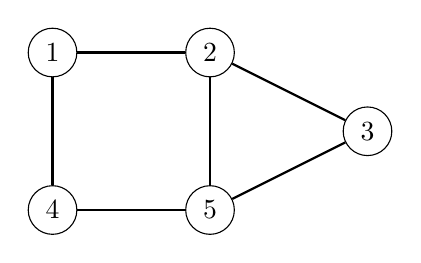
\begin{tikzpicture}
\node[draw, circle] (2) at (5,5) {$2$};
\node[draw, circle] (1) at (3,5) {$1$};
\node[draw, circle] (3) at (7,4) {$3$};
\node[draw, circle] (5) at (5,3) {$5$};
\node[draw, circle] (4) at (3,3) {$4$};

\path[draw,thick,-] (1) -- (2);
\path[draw,thick,-] (2) -- (5);
\path[draw,thick,-] (5) -- (4);
\path[draw,thick,-] (4) -- (1);
\path[draw,thick,-] (2) -- (3);
\path[draw,thick,-] (5) -- (3);
\end{tikzpicture}
\end{center}
Себебі, $1$-төбеден басталған тереңдігі бойынша ізденіс
былай жұмыс жасайды:
\begin{center}
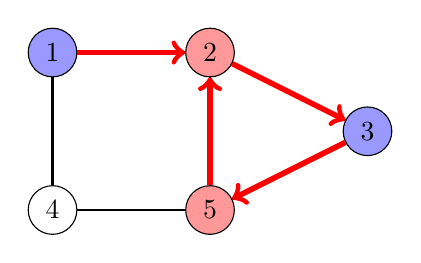
\begin{tikzpicture}
\node[draw, circle,fill=red!40] (2) at (5,5) {$2$};
\node[draw, circle,fill=blue!40] (1) at (3,5) {$1$};
\node[draw, circle,fill=blue!40] (3) at (7,4) {$3$};
\node[draw, circle,fill=red!40] (5) at (5,3) {$5$};
\node[draw, circle] (4) at (3,3) {$4$};

\path[draw,thick,-] (1) -- (2);
\path[draw,thick,-] (2) -- (5);
\path[draw,thick,-] (5) -- (4);
\path[draw,thick,-] (4) -- (1);
\path[draw,thick,-] (2) -- (3);
\path[draw,thick,-] (5) -- (3);

\path[draw=red,thick,->,line width=2pt] (1) -- (2);
\path[draw=red,thick,->,line width=2pt] (2) -- (3);
\path[draw=red,thick,->,line width=2pt] (3) -- (5);
\path[draw=red,thick,->,line width=2pt] (5) -- (2);
\end{tikzpicture}
\end{center}
Көріп отырғанымыздай үлгідегі граф екі ұялы емес. Себебі $2$ және $5$-төбелер
бірдей қызыл түске боялған, оған қоса көршілес келген.

Аталған алгоритм әрқашан да дұрыс жұмыс жасайды. Себебі графты екі түске бояған
кезде бастапқы төбе компоненттегі барлық басқа төбелердің
түстерін анықтайды.
Алғашқы төбенің қай түске, яғни қызылға немесе көкке боялғаны маңызды емес.

Басқа жағдайларда графты $k$ түске бояу мүмкіндігін тексеру
қиынға соғатынын ескергеніміз жөн. Тіпті $k=3$ деп алсақ та, әзірге тиімді алгоритм жоқ екенін айта кеткіміз келеді. 
Аталған есеп NP-қиын есептердің қатарына жатады.
